%%%%%%%%%%%%%%%%%%%%%%%%%%%%%%%%%%%%%%%%%%%%%%%%%%%%%%%%%%%%%%%%%%%
%%% Documento LaTeX 																						%%%
%%%%%%%%%%%%%%%%%%%%%%%%%%%%%%%%%%%%%%%%%%%%%%%%%%%%%%%%%%%%%%%%%%%
% T�tulo:		Cap�tulo 2
% Autor:  	Ignacio Moreno Doblas
% Fecha:  	2014-02-01
% Versi�n:	0.5.0
%%%%%%%%%%%%%%%%%%%%%%%%%%%%%%%%%%%%%%%%%%%%%%%%%%%%%%%%%%%%%%%%%%%
\chapterbegin{Trabajo Realizado} 

\label{chp:Utiliz}
%\minitoc
\section{Estudio basado en r�giones}
\par Uno de los principales problemas asociados al uso de redes de aprendizaje profundo son los altos costes de computaci�n y los amplios tiempos necesarios para la caracterizaci�n del algoritmo de aprendizaje, si son aplicados a datos de alta dimensionalida.
 
\begin{figure}[htp]
\centering
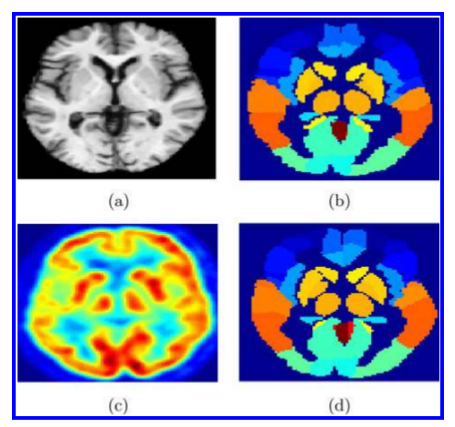
\includegraphics[scale=0.6]{images/img_4.png}
\caption{MRI image (a), MRI atlas (b), (c) PET image
and (d) PET atlas (same slice is shown in MRI and PET
images)}
\label{fig:CD_1}
\end{figure} 
 
\par Dada la alta dimensionalidad de las im�genes empleadas, en este estudio se ha realizado una aproximaci�n basada en r�giones, dado que las diferentes �reas cerebrales evaluadas tienen un tama�o considerablemente menor que las neuroim�genes enteras. No obstante, esta aproximaci�n tienes la ventaja de permitirnos caracterizar las r�giones por separado. 


\par Para la extracci�n de dichas r�gions de las neuroim�genes completas se ha empleado el atlas AAL (del ingl�s \textit{Automated Anatomical Labeling}). Este atlas permite obtener los v�xeles asociados a cada regi�n de manera normalizada.  


\par Dentro de estas r�giones normalmente aquellas a las que se les atribuye que aportan informaci�n sobre la detecci�n del AD se las denomina R�giones de Inter�s (ROI, del ingl�s \textit{Regions of Interest})

\section{Tratamiento de Neuroim�genes}
\subsection{Fuente de Datos}
\par Las neuroim�genes empleadas en este trabajo pertenecen a la iniciativa ADNI. Se han empleado tanto im�genes MRI como im�genes PET. Se disponen de 229 im�genes MRI de sujetos NC y 188 de sujetos de AD. Por otro lado, en el caso de las im�genes PET se disponen de 70 im�genes de sujetos AD y 68 de sujetos NC. 

\begin{table}[]
\centering
\label{my-label}
\begin{tabular}{ l | c | r | l | l } 
 Diagnosis & Number & Age &  Gender (M/F) & MMSE  \\ \hline
 Control & 68  &  75.81 $\pm$ 4.93 & 43/25 & 29.06 $\pm$ 1.08 \\ \hline
 AD & 70  & 73.06 $\pm$ & 46/24  & 22.84 $\pm$ 2.61  

\end{tabular}
 \caption{Datos Demogr�ficos Im�genes MRI}

\end{table}

sadfasdf
\newpage
\section{Modelos Generativos}
asddfasdf
\newpage
\section{Modelos de Clasificaci�n}
asdfasdf






































\chapterend{}